% Figure M10 hero prototype : generated by experiments/m10_agentic.py --hero.
% Preview-only; not yet linked from the main manuscript.
\begin{figure}[t]
 \centering
 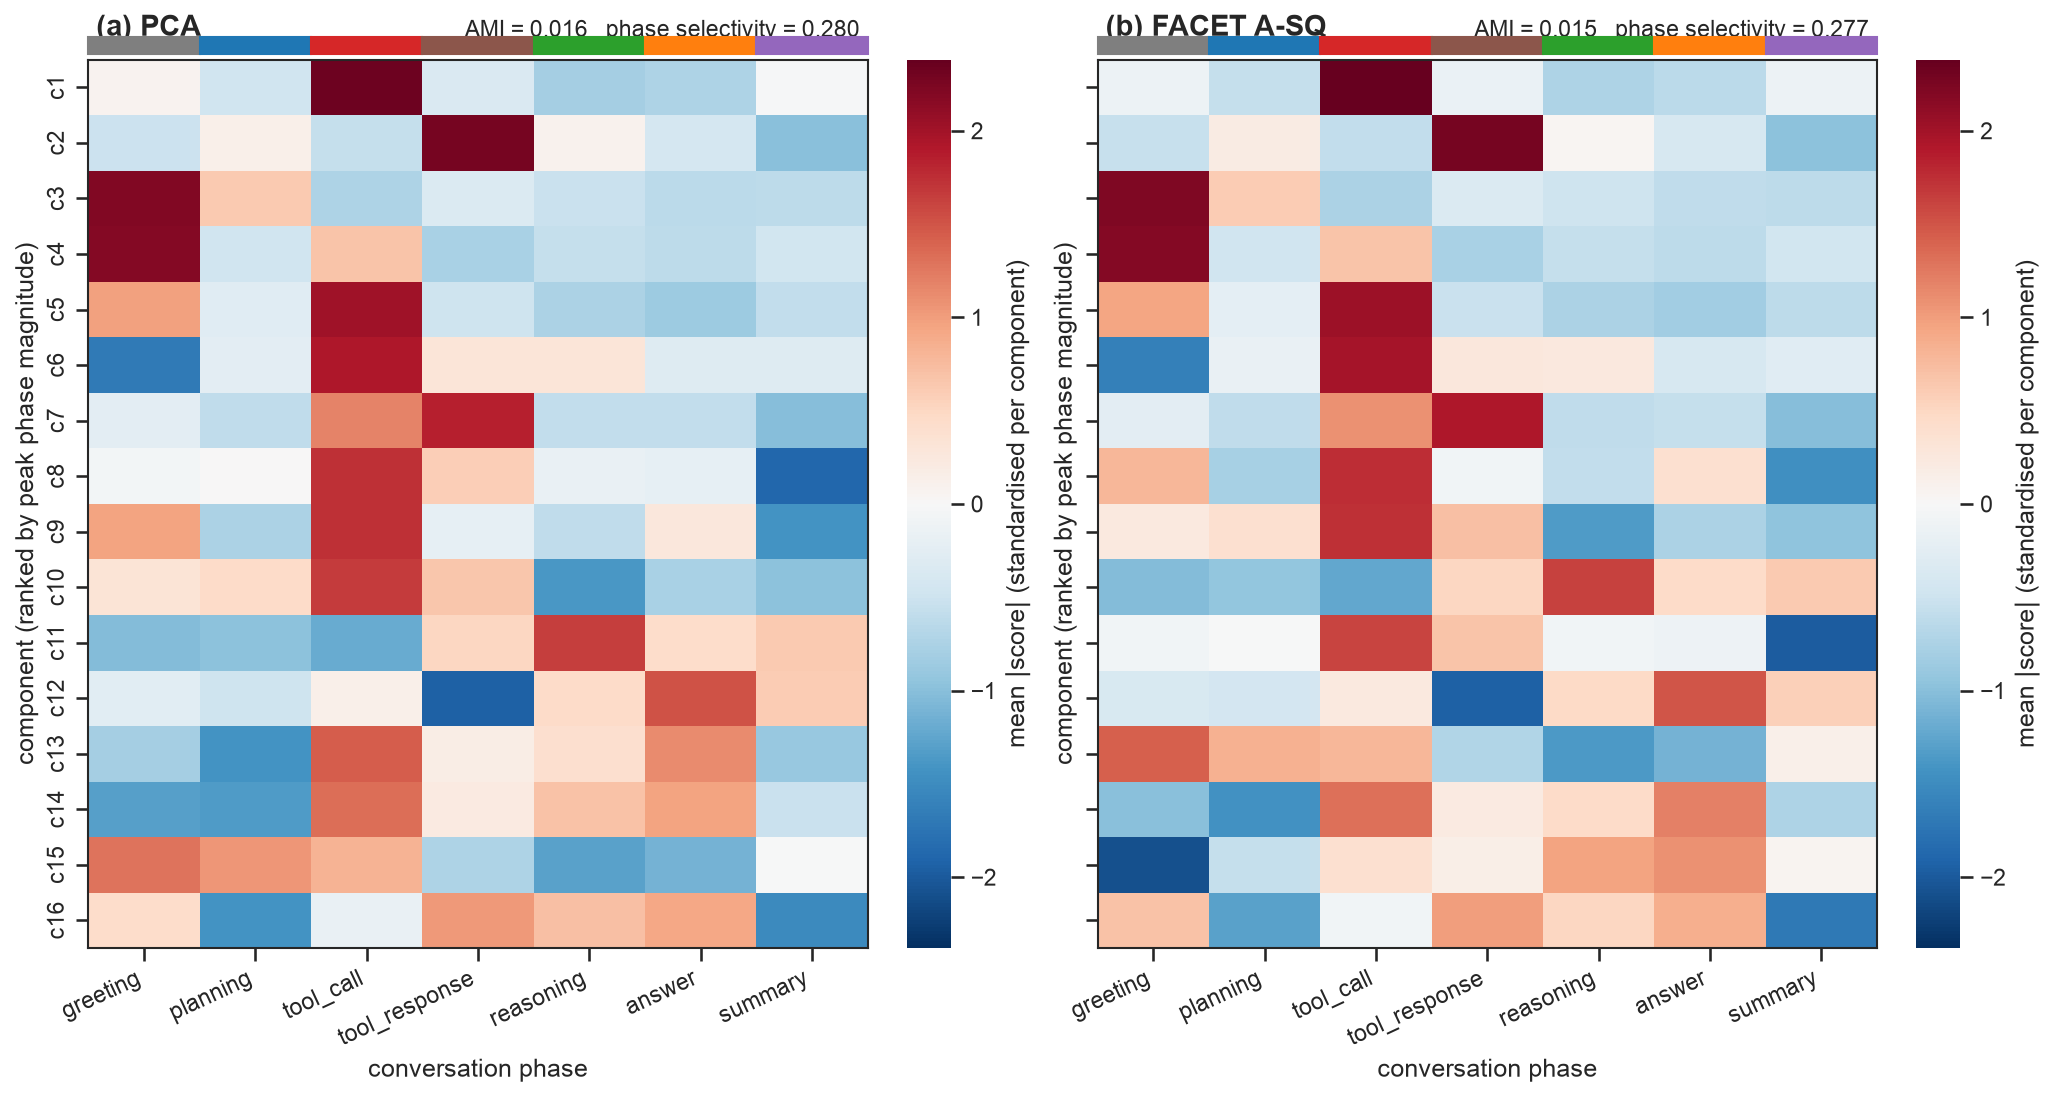
\includegraphics[width=\linewidth]{../shared/figures/generated/m10_agentic_hero.png}
 \caption{\textbf{M10: agentic AI, component--phase heatmap on multi-turn tool-use conversations.} Seven hand-written conversations alternate through \texttt{greeting}, \texttt{planning}, \texttt{tool\_call}, \texttt{tool\_response}, \texttt{reasoning}, \texttt{answer}, and \texttt{summary} phases ($836$ tokens total). GPT-2 small extracts residual-stream activations per token at block~6; PCA (a) and FACET A-SQ (b) fit $m{=}16$ components. Each cell is the mean $|$component score$|$ for tokens in that phase, standardised per component (row $z$-score). Rows are sorted by peak phase magnitude. The in-panel badges report the dominant-component AMI against the ground-truth phase label and the mean per-component ``phase selectivity'' $(\max - \mathrm{median})/\max$. FACET components concentrate activity on \texttt{tool\_call}, \texttt{tool\_response}, and \texttt{greeting} spikes (red/blue bands) while PCA spreads activity more uniformly across phases.}
 \label{fig:m10-agentic-hero}
\end{figure}
